\chapter[Vícerozměrný regresní model \\ Binární veličiny]{Vícerozměrný regresní model - binární veličiny}

Pro vyjádření kvalitativní veličiny se velmi často používá 
hodnot nula a jedna. Pomocí této tzv. binární veličiny (binary / dummy variable)
nejčastěji vyjadřujeme, zda-li pozorování náleží do určité 
skupiny, či nikoliv. Pomocí binární vysvětlující veličiny lze 
snadno rozšířit klasický regresní model.

\section{Binární veličina ve funkci průsečíku regresního modelu}

Jako příklad regresního modelu, do jehož průsečíku vstupuje 
binární veličina, uvažujme model
\begin{equation}
wage = \beta_0 + \delta_0 female + \beta_1 educ + u,
\end{equation}
který vyjadřuje závislost mezi mzdou a délkou vzdělání; 
binární veličina $female$ je rovno jedné, pokud se jedná o ženu, 
a nule, pokud se jedná o muže. Parametr $\delta_0$ tak vyjadřuje 
rozdíl mzdy muže a ženy za předpokladu stejného dosaženého 
vzdělání, tj.
\begin{equation}
\delta_0 = E[wage|female,educ] - E[wage|male, educ]
\end{equation}
a představuje tak posun průsečíku regresního modelu pro muže vs. ženy.

\begin{figure}[htp]
\centering
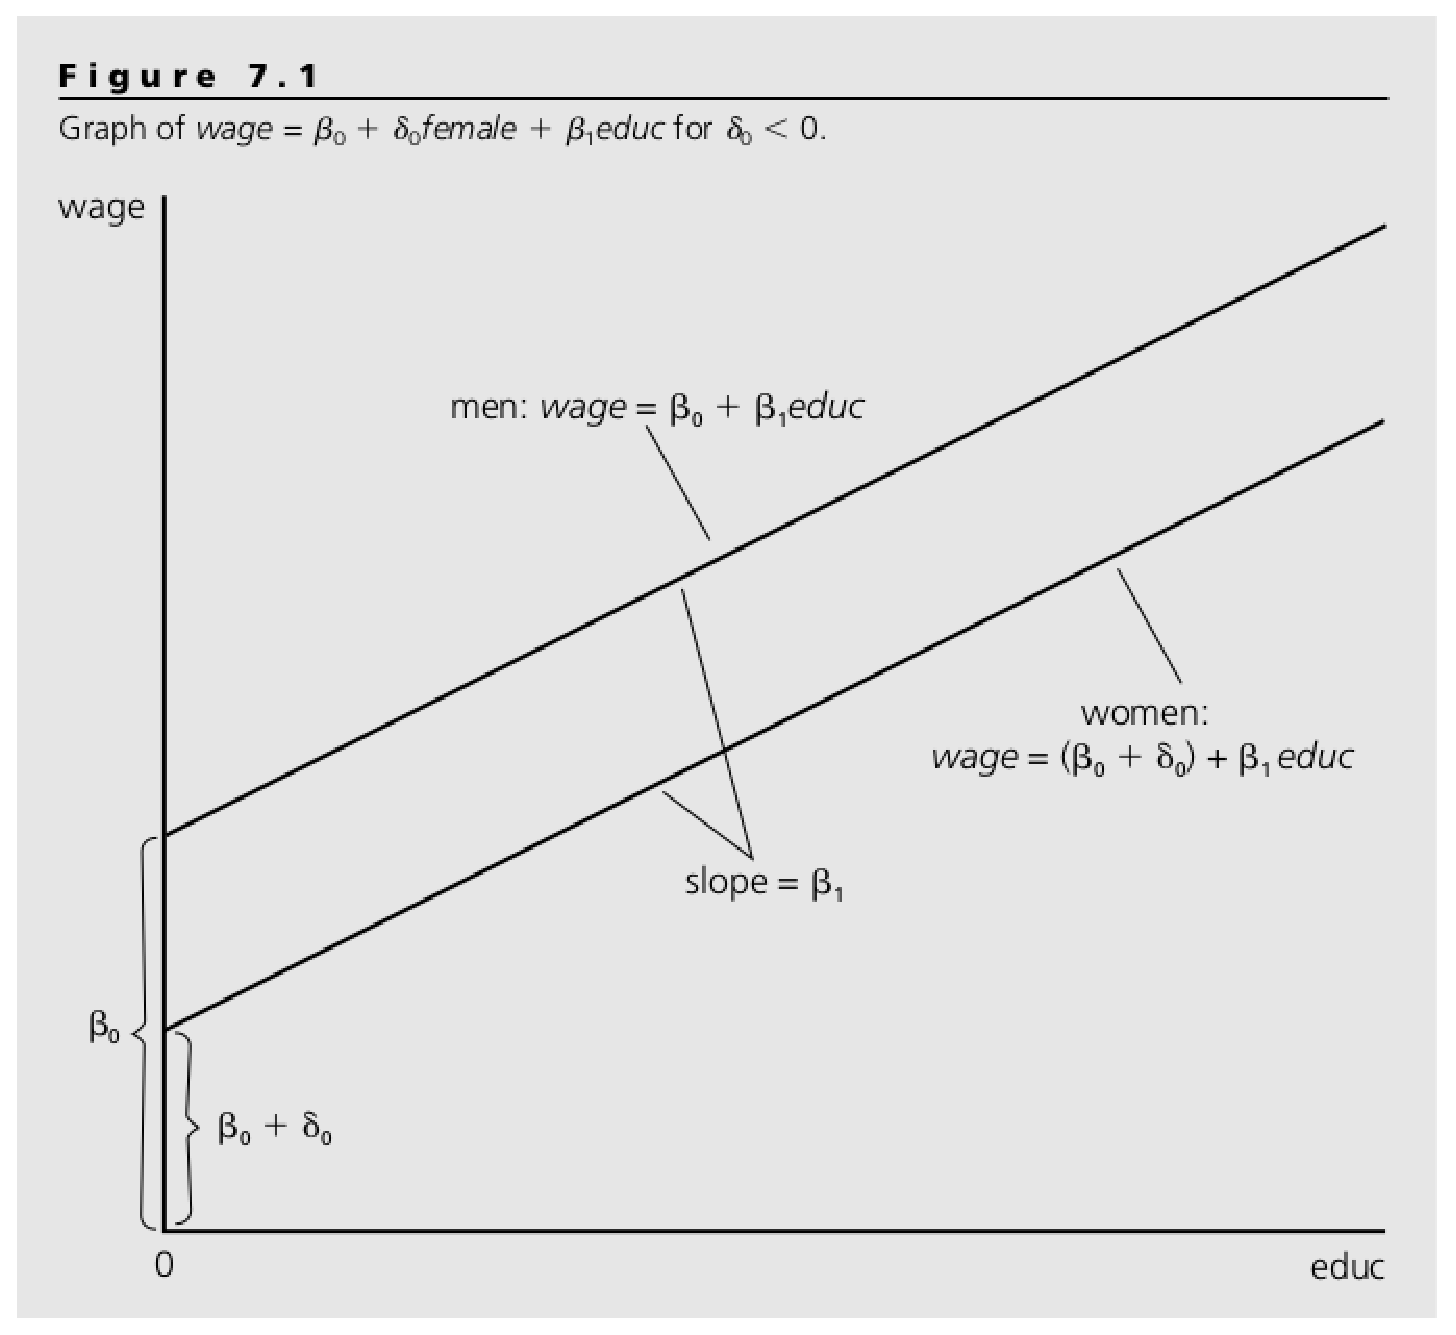
\includegraphics[scale = 0.5]{pictures/figure_7_1.eps}
\caption{Binární veličina a průsečík regresního modelu}
\label{figure_7_1}
\end{figure} 

Při používání binárních vysvětlujících veličin je třeba se 
vyvarovat tzv. pasti binární veličiny (dummy variable trap), která vede k již dříve 
diskutované dokonalé multikolinearitě. Té bychom se dopustili, 
pokud bychom regresní model (7.1) rozšířili do tvaru
\begin{equation}
wage = \beta_0 + \delta_0 female + \delta_1 male + \beta_1 educ + u,
\end{equation}
protože $female + male$ je vždy rovno jedné. Nic nám však nebrání 
tento model převést do tvaru
\begin{equation}
wage = \beta_0 + \delta_0 male + \beta_1 educ + u
\end{equation}
popř. do tvaru
\begin{equation}
wage = \delta_0 female + \delta_1 male + \beta_1 educ + u.
\end{equation}
V druhém případě jsme se vyhnuli pasti binární veličiny, 
protože jsme do modelu nezahrnuli obecný průsečík.

Testování parametru sklonu binárních veličin je stejné jako v 
případě testování sklonu standardních veličin, tj. pomocí $t$ 
testu. Aby byly závěry $t$ testu platné, musí být splněn 
předpoklad homoskedasticity, což znamená, že populační rozptyl 
příjmu mužů musí být stejný jako populační rozptyl příjmu žen.

V předchozím případě jsme uvažovali pouze dvě kategorie - muž a 
žena. Pokud však uvažujeme $n$ kategorií, je zapotřebí $n-1$ 
vysvětlujících binárních veličin.

\section{Regresní model zahrnující interakci binárních veličin}

Binární veličiny je možné mezi sebou také kombinovat. Jako 
příklad uvažujme regresní model
\begin{equation}
wage = \beta_0 + \delta_0 female + \delta_1 maried + \delta_2 female 
\cdot maried + \beta_1 educ + u.
\end{equation}
Tímto způsobem lze provést ``dekompozici'' průsečíku s ohledem na 
rodinný stav a pohlaví.

\section{Binární veličina ve funkci sklonu regresního modelu}

Binární veličiny lze snadno použít také jako ``modifikátor'' 
sklonu regresního modelu pro určitou vysvětlující veličinu. Pro 
ilustraci uvažujme model
\begin{equation}
wage = (\beta_0 + \delta_0 female) + (\beta_1 + \delta_1 female)educ + 
u
\end{equation}
resp. po roznásobení
\begin{equation}
wage = (\beta_0 + \delta_0 female) + \beta_1 educ + \delta_1 female \cdot educ + 
u,
\end{equation}
kde $\delta_0$ představuje rozdíl v průsečíku mezi muži a ženami 
a $\delta_1$ měří rozdíl v přínosu vzdělání mezi muži a 
ženami. Pokud by neexistovala mzdová diskriminaci podle pohlaví, pak 
by odhad jak $\delta_0$ tak $\delta_1$ byl statisticky 
nevýznamný.

\begin{figure}[htp]
\centering
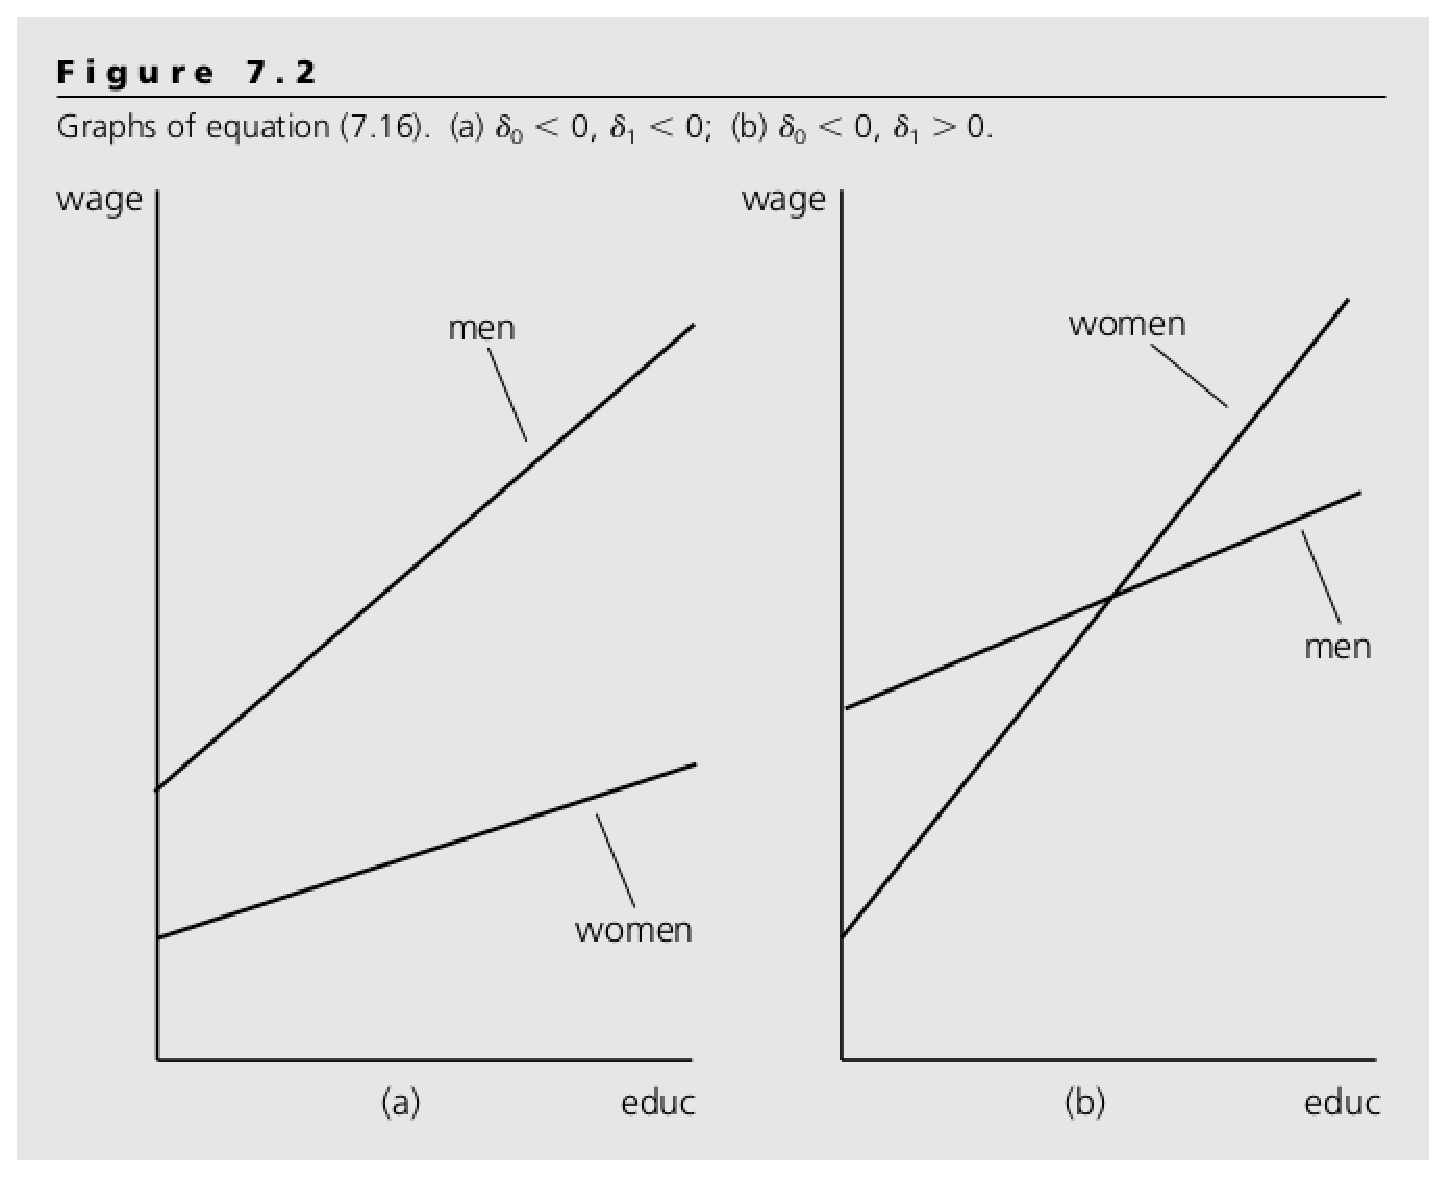
\includegraphics[scale = 0.5]{pictures/figure_7_2.eps}
\caption{Binární veličina a sklon regresního modelu}
\label{figure_7_2}
\end{figure} 

Pokud je zapotřebí testovat sdruženou významnost binárních 
veličin, tj. v našem případě nulovou hypotézu $H_0: \delta_0 = 0, 
\delta_1 = 0$, je možné použít modifikovaný $F$ test, který se 
nazývá Chowovým testem. Námi zkoumanou populaci rozdělíme na dvě 
subpopulace - na muže a ženy. Následně vypočteme $SSR_m$, $SSR_f$ 
a $SSR_P$ z odhadnutého regresního modelu pro muže
\begin{equation}
y = \beta_0^m + \beta_1^m educ + u,
\end{equation}
ženy
\begin{equation}
y = \beta_0^f + \beta_1^f educ + u
\end{equation}
a celou populaci
\begin{equation}
y = \beta_0^P + \beta_1^P educ + u.
\end{equation}
$F$ statistika je pak definována jako
\begin{equation}
F = \frac{SSR_P - (SSR_m + SSR_f)}{SSR_m + SSR_f} \frac{n - 2(k + 1)}{k 
+ 1}.
\end{equation}
Protože Chowovův test je $F$ testem, také on implicitně 
předpokládá splnění homoskedasticity, což znamená shodný rozptyl 
chybových členů pro obě subpopulace. Připomeňme, že pro účely asymptotické analýzy nemusí být 
splněn předpoklad normality.

\section{Lineární pravděpodobnostní model}

Uvažujme lineární pravděpodobnostní model (linear probability model)
\begin{equation}
y = \beta_0 + \beta_1 x_1 + ... + \beta_k x_k + u,
\end{equation}
kde $y$ má podobu binární veličiny. V tomto případě lze
\begin{equation}
E[y|x_1, ..., x_k] = \beta_0 + \beta_1 x_1 + ... + \beta_k x_k
\end{equation}
interpretovat je smyslu $P[y = 1|x_1, ..., x_k] = E[y | x_1, ..., 
x_k]$, tj. jako pravděpodobnost ``úspěchu''.

Pokud do odhadnutého regresního modelu
\begin{equation}
\hat{y} = \hat{\beta}_0 + \hat{\beta}_1 x_1 + ... + \hat{\beta}_k x_k
\end{equation}
dosadíme určité kombinace vysvětlujících veličin, může se 
stát, že predikovaná hodnota nebude spadat do intervalu nula až 
jedna, tj. bude v rozporu s jedním ze základním axiomů 
pravděpodobnosti. Tento problém lze např. vyřešit aplikací 
jednoduchého pravidla $\tilde{y}_j = 1$ pro $\hat{y}_j \ge 0.5$ a 
$\tilde{y} = 0$ pro $< 0.5$. Navzdory tomuto nedostatku je však lineární 
pravděpodobnostní model často aplikován v ekonomii. Tento model totiž 
často funguje relativně dobře pro nezávislé veličiny, jejichž 
hodnoty se nachází poblíž průměrných hodnot.

Kvůli binární povaze vysvětlované veličiny $y$ je porušen jeden 
z Gaus-Markovových předpokladů. Jestliže je $y$ binární veličinou, 
pak je její podmíněný rozptyl roven
\begin{equation}
var[y|x] = p(x)\left(1 - p(x)\right),
\end{equation}
kde $p(x)$ představuje pravděpodobnost úspěchu $p(x) = \beta_0 + 
\beta_1 x_1 + ... + \beta_k x_k$. Protože $p(x)$ je funkcí 
vysvětlujících veličin, musí být nutně porušen předpoklad 
homoskedasticity. Připomeňme, že homoskedasticita je nezbytná pro 
platnost $t$ a $F$ statistik. Proto je třeba směrodatné 
odchylky odhadnutých parametrů používat opatrně. V následující kapitole
si představíme směrodatnou odchylku, která je vzhledem k možné 
heteroskedasticitě robustní. Navíc si také ukážeme, že v praxi 
mnohdy nepředstavuje heteroskedasticita zásadní problém, a že 
standardní OLS statistiky jsou stále použitelné. 
